\documentclass[../main.tex]{subfiles}

\begin{document}
Sabiendo que:
\begin{align}
  F &= -kx \nonumber \\
  mg &= -kx \nonumber \\
  \abs{mg} &= \abs{-kx} \nonumber \\
  \label{eq:elastiK}
  k &= \frac{\abs{mg}}{\abs{x}} = \frac{\abs{F}}{\abs{x}}
\end{align}
Donde $m$ es la masa del objeto, $g$, el módulo de la gravedad, y $x$ el desplazamiento del resorte respecto de su longitud natural.
Para determinar el peso del objeto $mg$, es preciso realizar la conversión de unidades de gramos y centímetros, a kilogramos y metros respectivamente.
Cabe resaltar la consideración de 4 cifras significativas en el valor de la aceleración de la gravedad, siendo esta de \qty{9.807}{\metre\per\second\squared}.
\begin{table}[H]
  \caption{Medida de la elongación total del resorte en función de las masas combinadas}
  \label{tab:massToLength}
  \begin{center}
    \begin{tabular}[c]{lrr}
      \toprule
      \multicolumn{1}{c}{Número de combinación} &
      \multicolumn{1}{c}{Masa de combinación (\unit{\gram})} &
      \multicolumn{1}{c}{$L_0 + \Delta L (\pm \qty{0.05}{cm})$} \\
      \midrule
      1 & \num{515.2 +- 0.1} & \num{29.00} \\
      2 & \num{717.4 +- 0.2} & \num{34.90} \\
      3 & \num{767.1 +- 0.2} & \num{36.40} \\
      4 & \num{969.3 +- 0.3} & \num{42.40} \\
      5 & \num{1526.7 +- 0.2} & \num{58.50} \\
      \bottomrule
    \end{tabular}
  \end{center}
\end{table}
\begin{figure}
  \begin{center}
    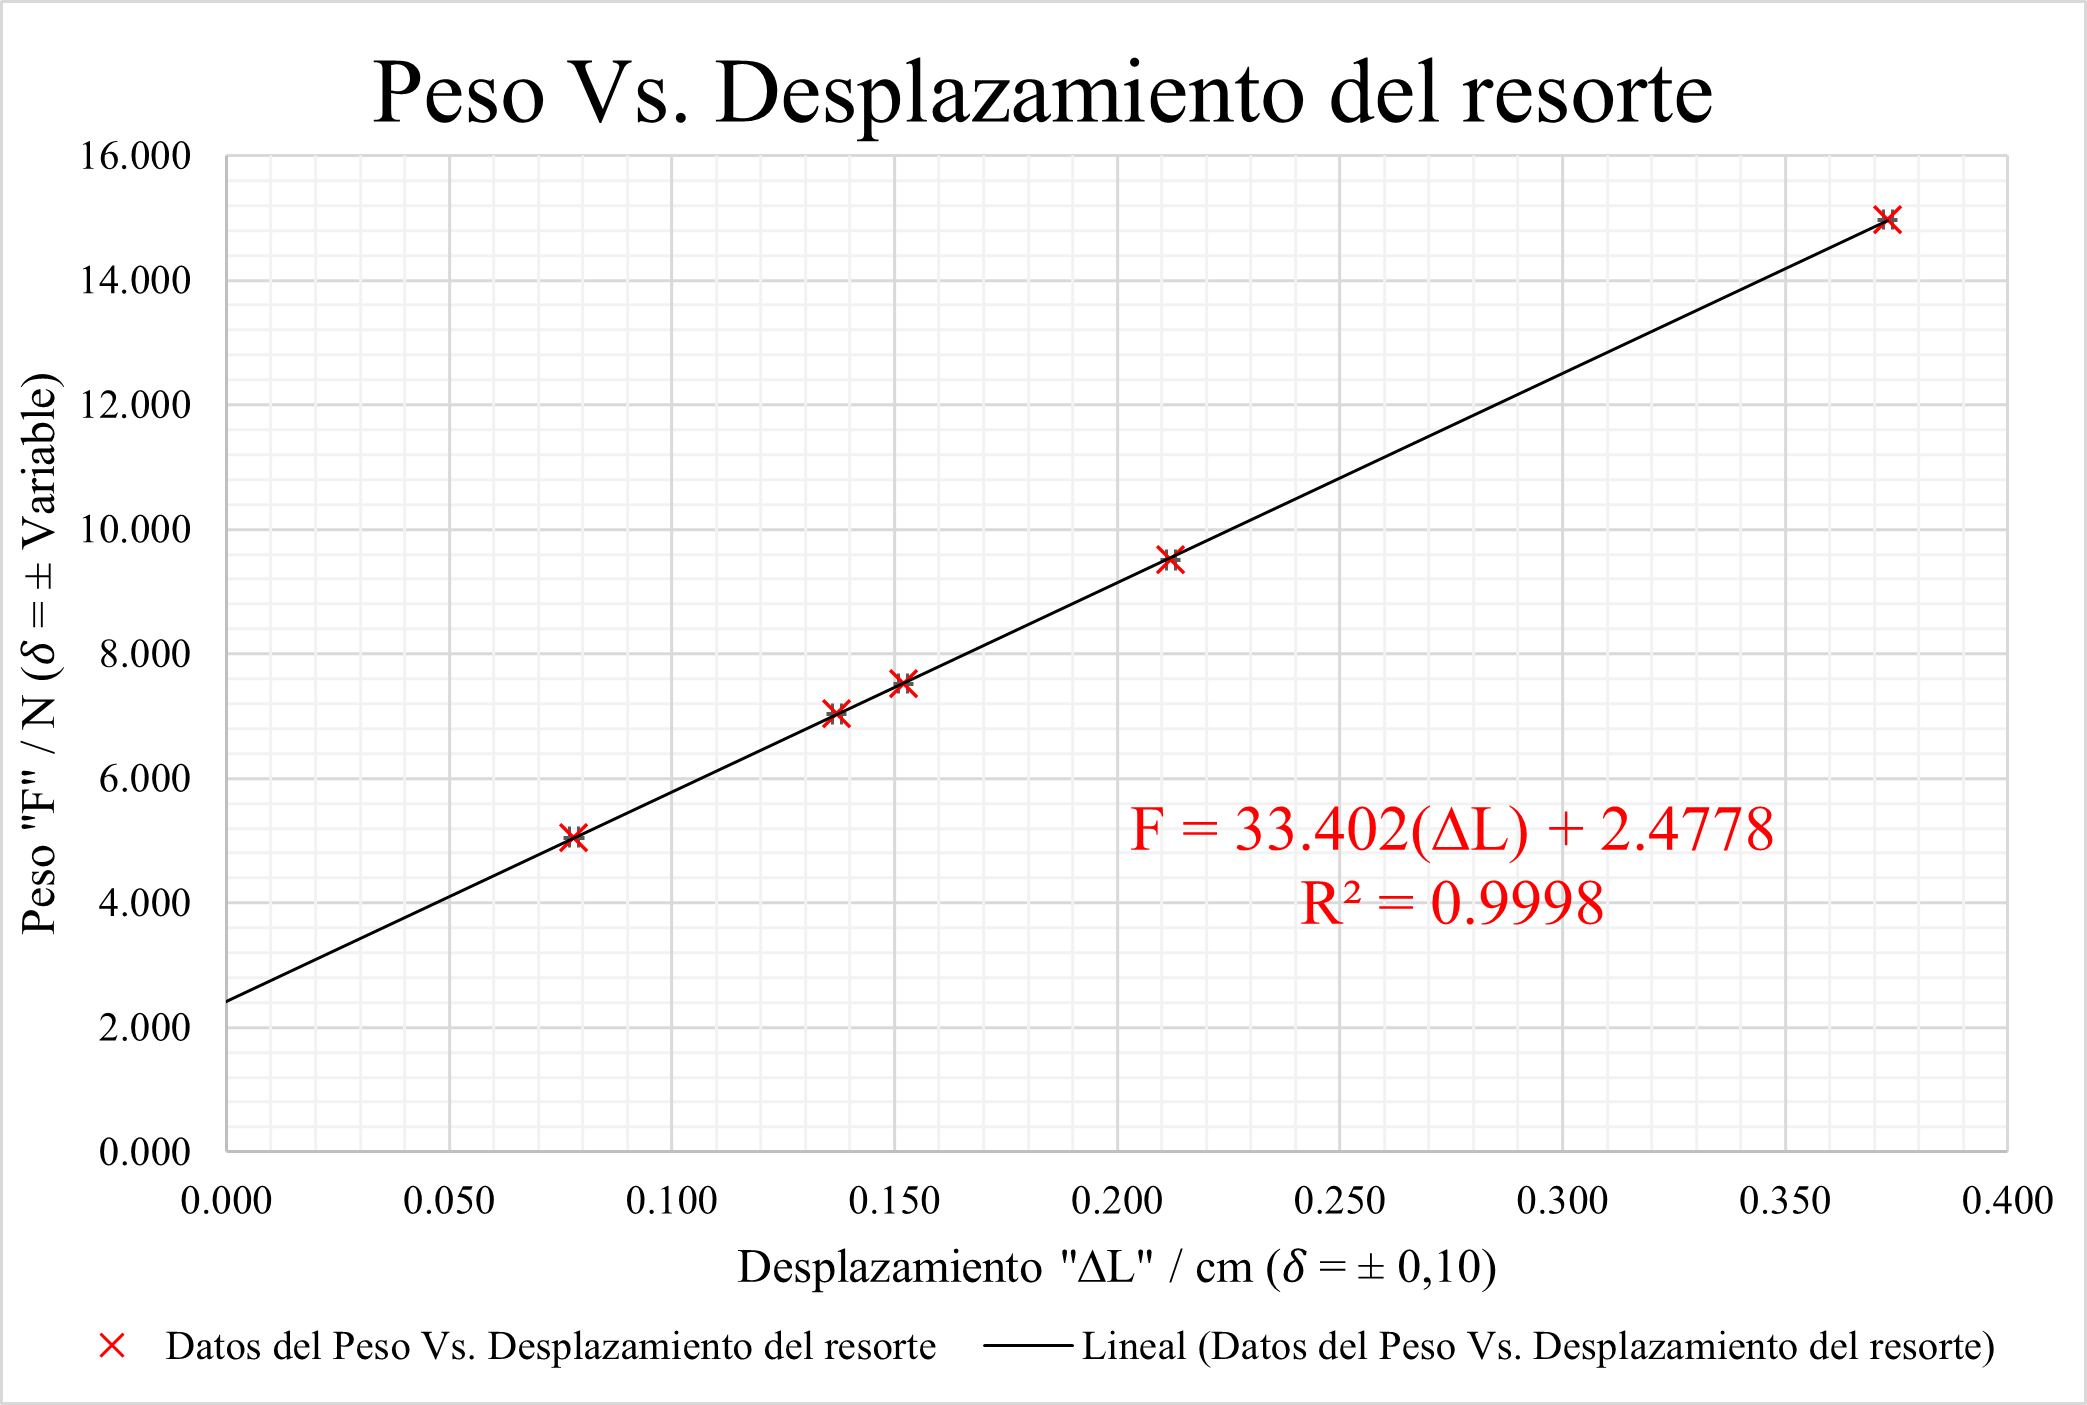
\includegraphics[width=0.95\textwidth]{resources/resl1.png}
  \end{center}
  \caption{Relación entre el peso de los cuerpos y el desplazamiento del resorte}
  \label{fig:weightAndDelta}
\end{figure}
De la gráfica 1, se puede observar en primer lugar, que el ajuste de la recta es bastante preciso, esto se puede comprobar verificando que el coeficiente determinación (R2), es aproximadamente la unidad, evaluado en el orden de las diezmilésimas.

Además, las barras de error en ambas dimensiones son prácticamente despreciables en relación a la escala representada en la gráfica 1.

Luego, de la ecuación señalada, es posible extraer su pendiente, la cual representa la constante K del resorte de acuerdo al ajuste por mínimos cuadrados realizado.
\begin{equation}
  F = \num{33.402} (\Delta L) + \num{2.4778}
  \label{eq:linearModel}
\end{equation}
En primera instancia, se observa en la ecuación \ref{eq:linearModel}, un término independiente que es igual al peso cuando el desplazamiento del resorte respecto a la longitud natural es igual a cero.
Visto desde un punto de vista físico, la existencia de este término puede deberse a errores experimentales como la medición de los datos, la fricción y la resistencia del aire, que reducen la energía del sistema, afectando la relación entre los parámetros estudiados e introduciendo un término independiente en la ecuación.
Otra razón es que los resortes reales, no son perfectamente lineales, y pueden tener algunas irregularidades en su comportamiento, que se manifiestan en mayor medida, cuando el desplazamiento es muy grande, puesto que el material del resorte no es el más idóneo y su geometría no es perfectamente lineal.
Por otro lado, al evaluar $F = 0$, el desplazamiento toma un valor negativo, que representa una compresión del resorte en dirección opuesta a la atracción gravitatoria.

De la ecuación \ref{eq:linearModel}, el valor de la constante K del resorte es \qty{33.40}{\newton\per\metre}, redondeado a 4 cifras significativas de acuerdo a las cifras significativas de los datos tomados experimentalmente.

Posteriormente, con el objetivo de determinar la incertidumbre asociada, se utilizó el software Excel, reconocido por su capacidad en el análisis de datos y cálculos precisos. Como resultado de dicho análisis, se obtuvo un valor de \qty{0.26}{\newton\per\metre} para la magnitud en cuestión. Entonces:
\begin{equation*}
  K \pm \Delta K = \qty{33.40 +- 0.26}{\newton\per\metre}
\end{equation*}
Evaluando la incertidumbre relativa de K:
\begin{equation*}
  \varepsilon_R = \frac{\Delta K}{K} = \frac{\num{0.26}}{\num{33.40}} \approx \qty{0.78}{\percent}
\end{equation*}
El error relativo es incluso menor a \qty{1}{\percent}, lo cual indica una alta precisión de la medida, atribuyéndole una mayor confiabilidad al realizar cálculos futuros con la misma.
\begin{table}[H]
  \caption{Relación entre la frecuencia y el tiempo requerido para completar 10 oscilaciones en función de diferentes masas y amplitudes}
  \label{tab:massAndFreq}
  \begin{center}
    \begin{tabular}[c]{lrrrrr}
      \toprule
      \multirow{2}{*}{Número de combinación} &
      \multicolumn{4}{c}{$\Delta t \qty{+- 0.01}{\second}$} &
      \multirow{2}{*}{$\mathit{v} \, (\unit{osc\per\second})$} \\
      \cmidrule{2-4}
      & $\Delta t_1$ & $\Delta t_2$ & $\Delta t_3$ & $\Delta t_4$ & \\
      \midrule
      1 & \num{7.92} & \num{7.94} & \num{7.93} & \num{7.93} & \num{1.26} \\
      2 & \num{9.37} & \num{9.37} & \num{9.36} & \num{9.37} & \num{1.07} \\
      3 & \num{9.62} & \num{9.57} & \num{9.53} & \num{9.57} & \num{1.04} \\
      4 & \num{10.88} & \num{10.86} & \num{10.85} & \num{10.86} & \num{0.9208 +- 0.0008} \\
      5 & \num{13.55} & \num{13.60} & \num{13.54} & \num{13.56} & \num{0.7375 +- 0.0005} \\
      \bottomrule
    \end{tabular}
  \end{center}
\end{table}
En la tabla \ref{tab:massAndFreq}, se omitieron las incertidumbres de las masas 1, 2 y 3, puesto que su valor se encuentra debajo del orden del último decimal de cada una de esas tres masas, siendo irrelevantes para interpretar los resultados.

Sabiendo que, la frecuencia para un movimiento armónico simple (MAS) se rige por la siguiente ecuación derivada de la ecuación fundamental:
\begin{equation}
  \mathit{v} = \frac{1}{2\pi} \sqrt{\frac{F}{mx}}
  \label{eq:harmoFreq}
\end{equation}
Reemplazando \ref{eq:elastiK} en \ref{eq:harmoFreq}:
\begin{equation}
  \mathit{v} = \frac{1}{2\pi} \sqrt{\frac{k}{m}}
  \label{eq:harmoK}
\end{equation}
Luego, para determinar la incertidumbre de la frecuencia:
\begin{equation*}
  \mathit{v} \pm \Delta \mathit {v} = \frac{1}{2\pi} \sqrt{\frac{k \pm \Delta k}{m \pm \Delta m}}
\end{equation*}
Dado que el valor de $\pi$ es una constante matemática, y por tanto no tiene incertidumbre asociada, entonces:
\begin{align}
  \Delta \mathit{v} &= \sqrt{\frac{k}{m}\Bigl[\abs{1}\Bigl(\frac{\Delta k}{k}\Bigr) + \abs{-1}\Bigl(\frac{\Delta m}{m}\Bigr)\Bigr]} \nonumber \\
  &= \sqrt{\frac{k}{m} \Bigl(\frac{m \Delta k + k \Delta m}{km}\Bigr)} \nonumber \\
  &= \sqrt{\frac{m \Delta k + k \Delta m}{m^2}}
  \label{eq:freqDone}
\end{align}

Entonces, empleando la ecuación \ref{eq:harmoK} para determinar el valor absoluto de la frecuencia, y la ecuación \ref{eq:freqDone} para su incertidumbre:
\begin{table}[H]
  \caption{Relación entre las diferentes masas y la frecuencia del resorte, calculada utilizando una ecuación derivada del Movimiento Armónico Simple (MAS)}
  \label{tab:theoreticalMeasurements}
  \begin{center}
    \begin{tabular}[c]{lrr}
      \toprule
      \multicolumn{1}{c}{Número de combinación} &
      \multicolumn{1}{c}{Masa de combinación (\unit{\kilo\gram})} &
      \multicolumn{1}{c}{$\mathit{v^\prime} \, (\unit{osc\per\second})$} \\
      \midrule
      1 & \num{0.5152 +- 0.0001} & \num{1.281 +- 0.719} \\
      2 & \num{0.7174 +- 0.0002} & \num{1.086 +- 0.613} \\
      3 & \num{0.7671 +- 0.0002} & \num{1.050 +- 0.592} \\
      4 & \num{0.9693 +- 0.0003} & \num{0.9343 +- 0.5281} \\
      5 & \num{1.5267 +- 0.0002} & \num{0.7444 +- 0.4161} \\
      \bottomrule
    \end{tabular}
  \end{center}
\end{table}
Nótese que se ha empleado el mismo símbolo, pero primado para representar la frecuencia, de manera que, pueda diferenciarse entre el valor obtenido experimentalmente (véase tabla \ref{tab:massAndFreq}), y aquel determinado con la ecuación \ref{eq:harmoK}. (véase tabla \ref{tab:theoreticalMeasurements}).

Determinando el error relativo para las frecuencias de cada masa según la tabla 6, se obtiene:
\begin{equation*}
  \varepsilon_R = \frac{\Delta \mathit{v^\prime}_i}{\mathit{v'}_i}
\end{equation*}
\begin{table}[H]
  \caption{Errores relativos de las frecuencias determinadas para cada combinación de masa}
  \label{tab:theoError}
  \begin{center}
    \begin{tabular}[c]{lr}
      \toprule
      \multicolumn{1}{c}{$\mathit{v^\prime} \,$ (\unit{osc\per\second})} &
      \multicolumn{1}{c}{$\varepsilon_R$} \\
      \midrule
      \num{1.281 +- 0.719} & \num{0.561} \\
      \num{1.086 +- 0.613} & \num{0.564} \\
      \num{1.050 +- 0.592} & \num{0.564} \\
      \num{0.9343 +- 0.5281} & \num{0.5652} \\
      \num{0.7444 +- 0.4161} & \num{0.5590} \\
      \bottomrule
    \end{tabular}
  \end{center}
\end{table}
\end{document}
